\chapter{相关研究介绍}
本文的研究对象涉及自然语言处理的多个子领域,本章将分领域分别介绍歌曲歌词生成及限制性翻译和歌声合成相关技术的研究现状和近期进展。
歌曲歌词生成及限制性翻译目前有多个技术路线,分别着重于对自回归翻译的不同阶段施加限制,另外也有一些条件性歌词生成和对齐的相关技术与自动歌曲翻译这一任务相关。
歌声合成技术自语音合成发展而来,在语音合成方面,许多工作尝试以各类合成模型为基础搭建声学模型。这些模型因各自原理和结构不同,在模型规模、推理速度、训练难易度和合成表现上也各有千秋。
以下分别对这些子领域进行阐述。
\section{歌曲歌词生成及限制性翻译研究介绍}
歌词自动翻译研究历经基于规则的方法的阶段、统计机器翻译方法阶段和使用具有节奏和词汇句法约束的有限状态机阶段\citep{spanish_verse, Manurung2004AnEA, He_Zhou_Jiang_2012},近年来也逐渐开始引入神经网络模型向神经机器翻译靠拢
\citep{ghazvininejad-etal-2016-generating,ghazvininejad-etal-2017-hafez, ghazvininejad-etal-2018-neural}。
在语言学研究中,传统人工歌曲翻译研究通过利用语言学知识在歌词翻译和歌词旋律对齐方面都取得了一些进展
~\citep{interplay_lyrics_melody,low_2003,low2008translating,low_2022,three_d_of_singability,trans_of_music}.
当然,这些研究针对的对象都是专业歌手创作的歌曲,这些方法追求在一些有代表性的曲目中进行高质量的歌词翻译和歌词旋律对齐,力求达到``信、达、雅''的三重境界。
\begin{figure}[htbp]
  \centering
  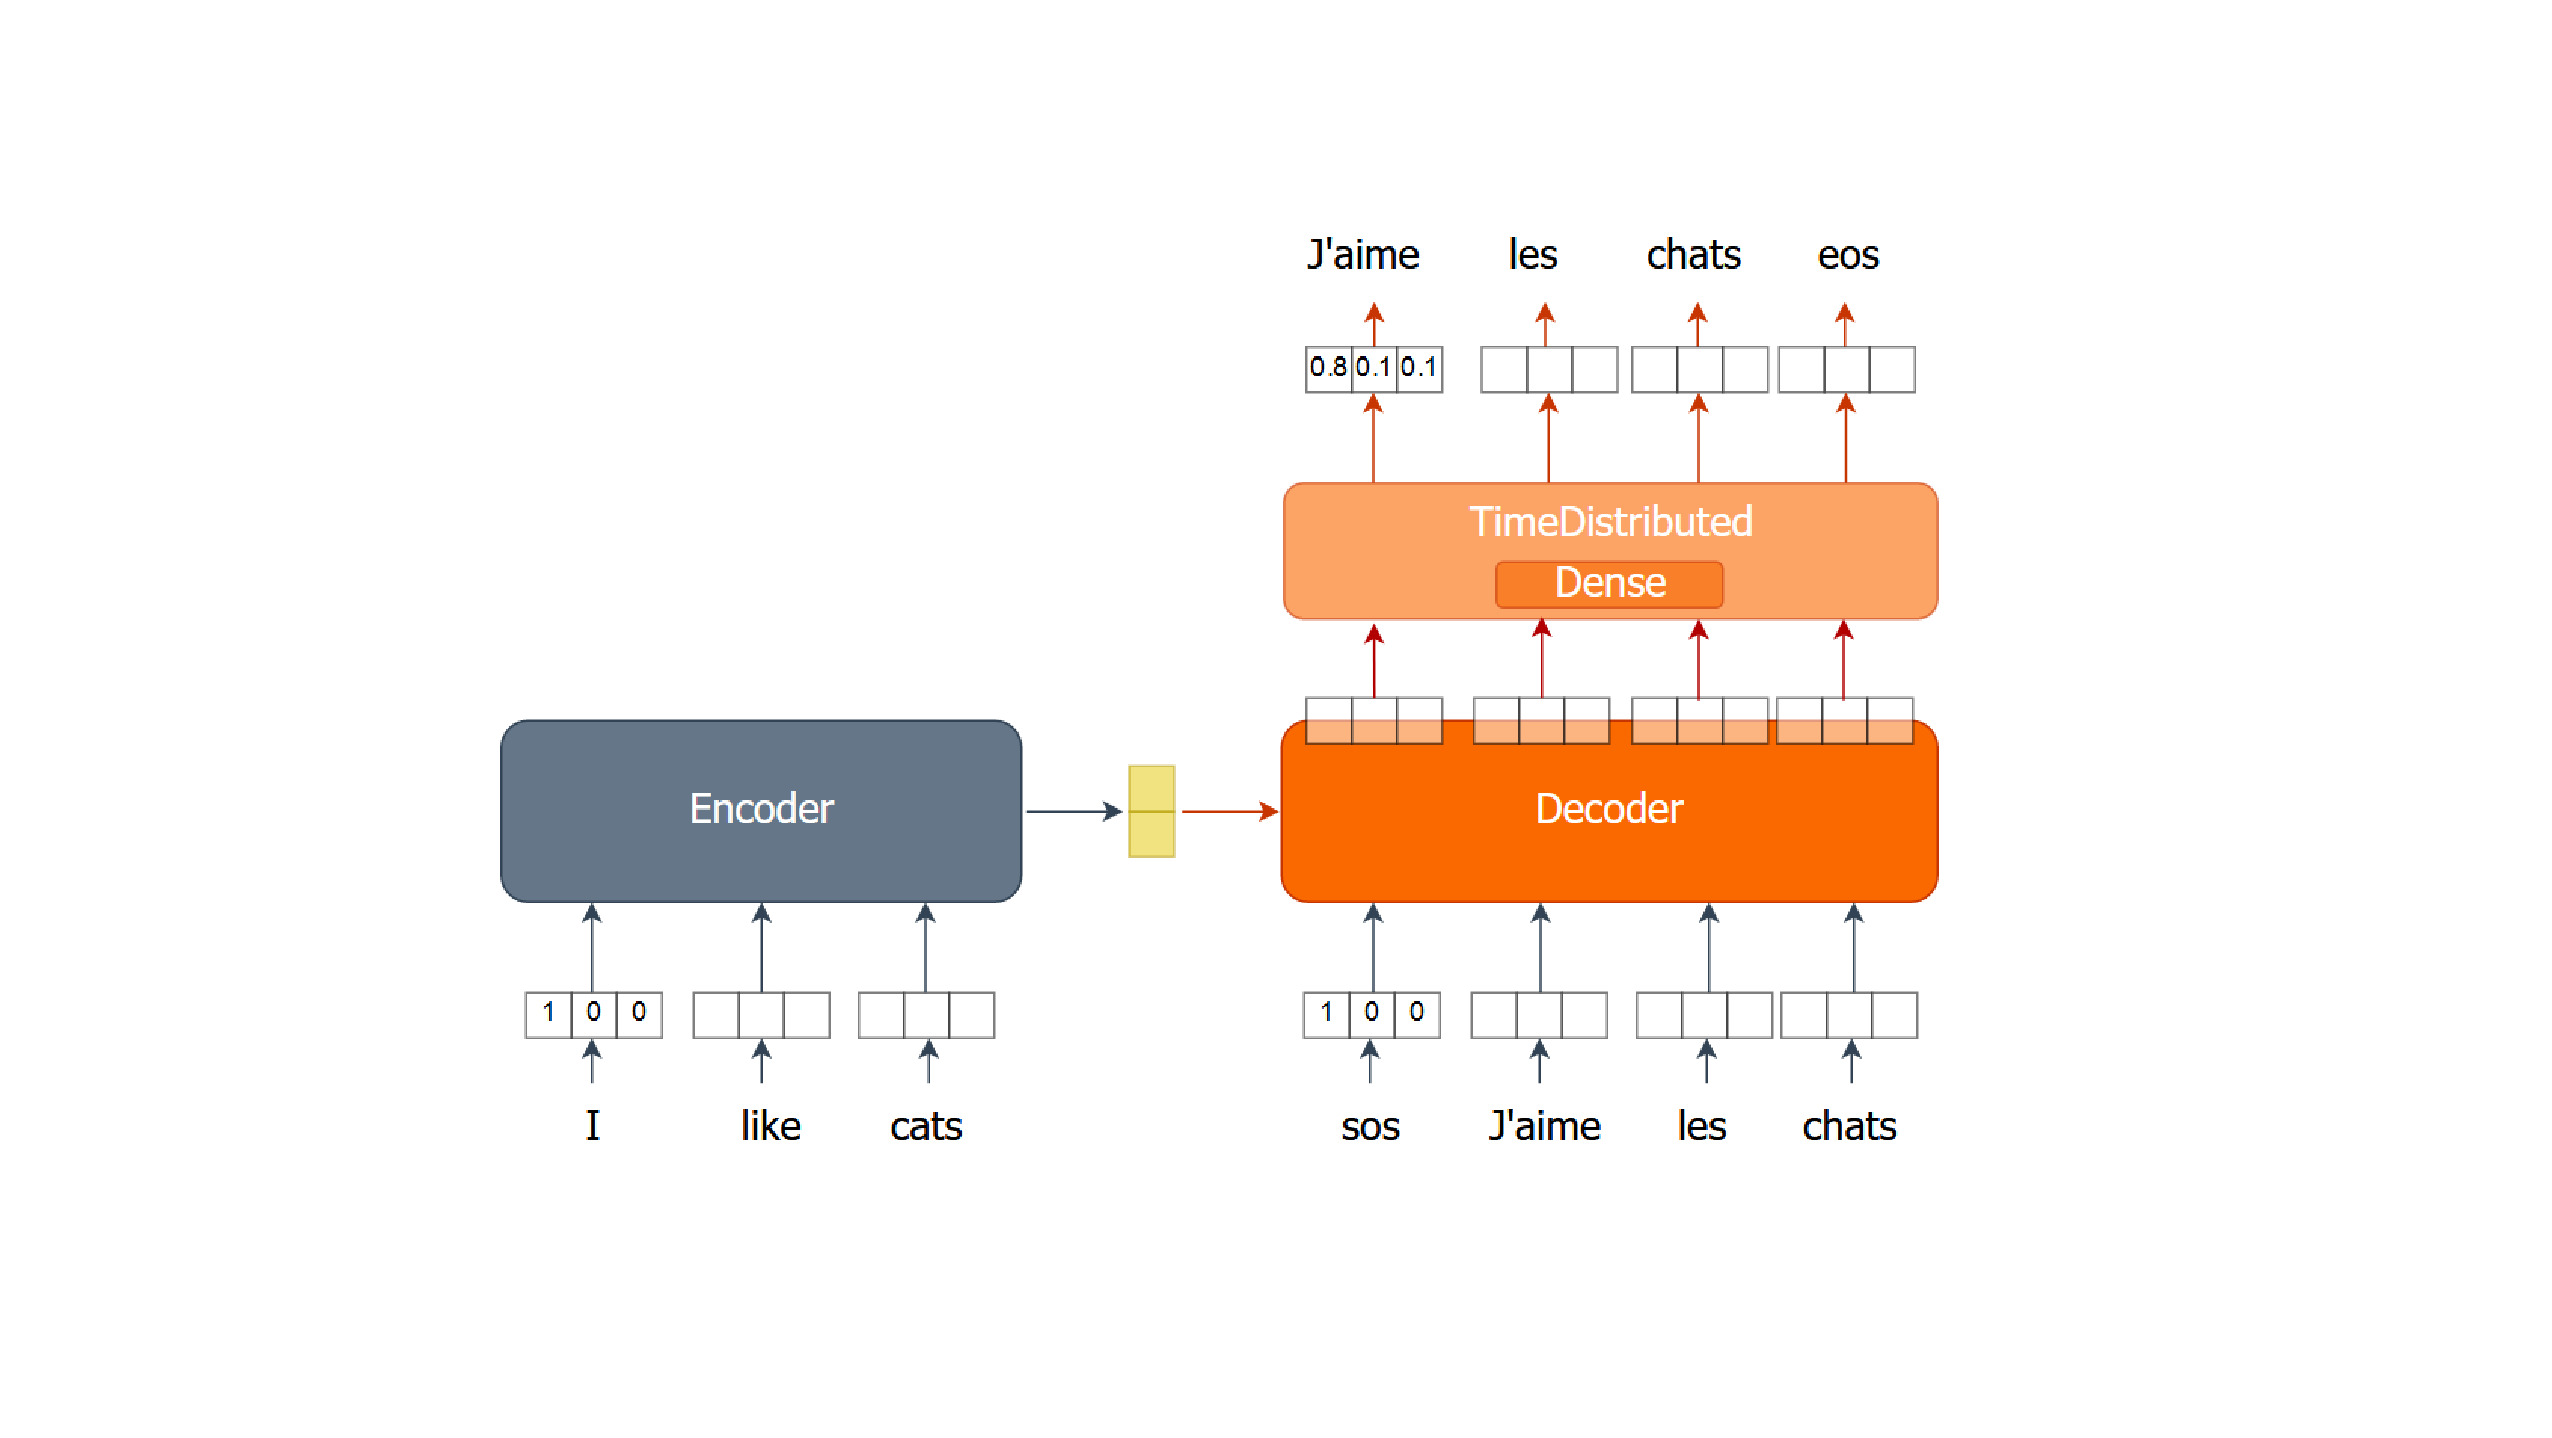
\includegraphics[width=0.99\textwidth]{figure/related/teacher-forcing.pdf}
  \caption{Teacher-forcing训练方式图示}
  \label{fig:tf_train}
\end{figure}
\subsection{基于序列生成的歌词生成、限制性生成和翻译}
\subsubsection{限制性生成和翻译研究}
在近来基于神经机器翻译的工作\citep{gagast}中,自动歌曲翻译大多被当作一种存在一定限制条件的文本翻译任务进行建模。目前,文本翻译作为一种序列生成任务,大都采用自回归式的解码方式,而以Teacher-forcing方式进行训练以加快收敛。
基于此,很多工作~\citep{hokamp-liu-2017-lexically,lakew-etal-2019-controlling,li-etal-2020-rigid,zou_controllable}尝试仅在解码过程中直接对解码搜索时的评分施加目的性限制来进行重评分,让符合限制的结果得分更高,不符合的得分减少。如限制符合诗词格式、限制符合某些语法规则等。
解码时对结果的评分原本只有来自神经网络训练出的语言模型根据编码器的输入和已经解码出的前文对当前位置应解码结果的概率估计:
\begin{equation}
  P(y_t|y_0,y_1......y_{t-1}, X)
\end{equation}
现在则需要根据是否符合限制的判断进行重评分:
\begin{equation}
  P(y_t|y_0,y_1......y_{t-1}, X)+f(y_0,y_1......y_{t-1}, \mbox{restrictions})
\end{equation}
xxx中使用
\begin{figure}[htbp]
  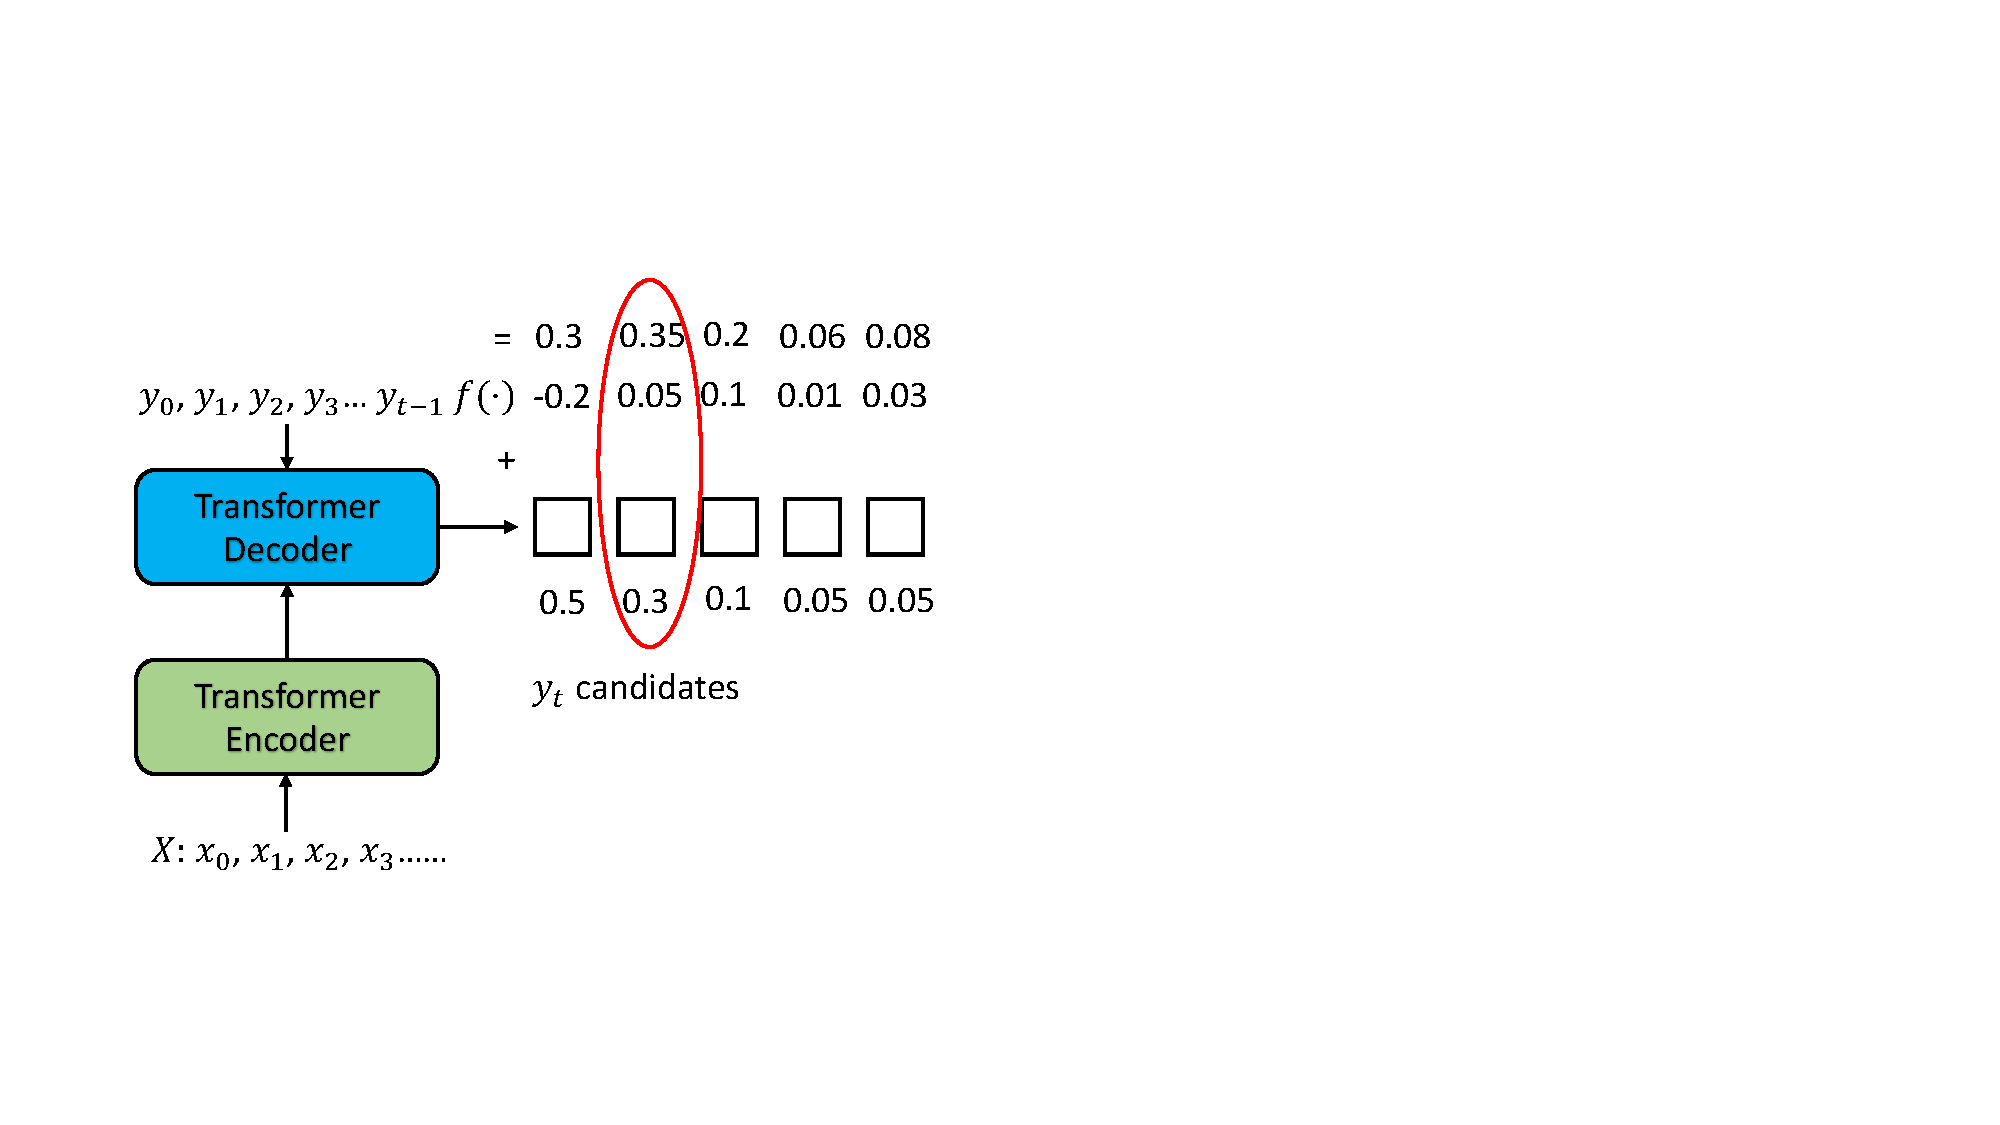
\includegraphics[width=0.99\textwidth]{figure/related/decoded_constrain.pdf}
  \caption{title}
\end{figure}
此方面工作的探索证明了这类比较直接的做法大部分都比较有效,而且对于一些本质比较简单的限制来说,这种做法所需的编码工作量小,实施起来非常方便,而且无需对已经训练好的神经网络模型做其他调整。

除此之外,很多工作尝试在训练过程中施加约束,如在输入中添加与格式限制有关的嵌入表示进行监督以在推理时控制解码~\citep{li-etal-2020-rigid}、引入特殊词语以达到长度控制的目的~\citep{lakew-etal-2019-controlling,saboo-baumann-2019-integration}等。这些方法通过在输入时引入额外的条件作为控制信息,在训练时通过相应的结果监督来使得模型依赖控制信息对最终结果产生的影响,进而在推理时通过提供不同的控制信息来控制解码结果。这些数据驱动的方法同样表现出良好的性能,且能施加更加复杂的限制,模型表现更可靠。但是和仅干预解码过程的做法相比,限制的变动都需要设计和训练模型学习限制的方式。
% \begin{figure}[htbp]
%   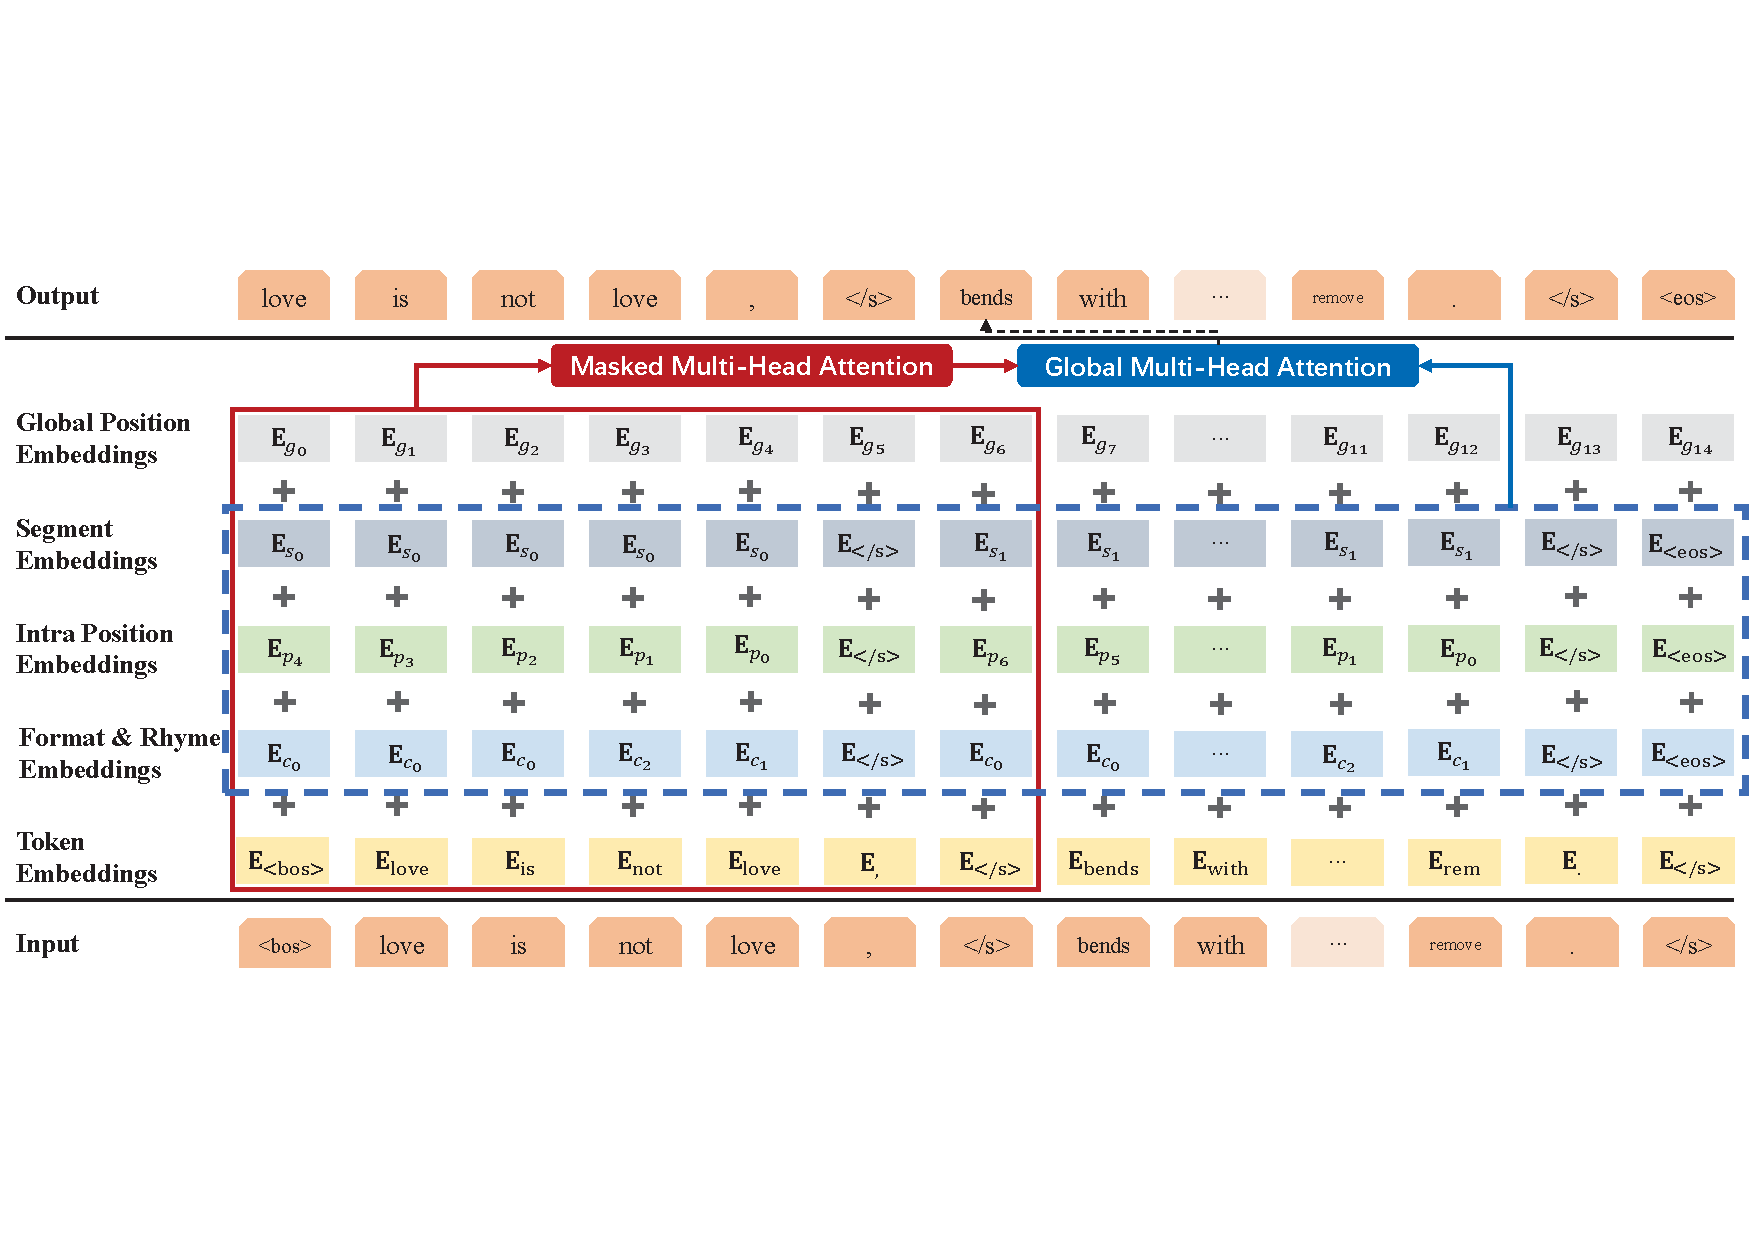
\includegraphics[width=0.99\textwidth]{figure/related/train_constrain.pdf}
%   \caption{title}
% \end{figure}
\subsubsection{自动歌词生成研究}


在下一章中,本文将提出歌词旋律对齐和歌词共同翻译模型,在翻译的语料上进行翻译域偏移适应,同时也对翻译文本结果进行长度限制。
\subsection{歌词-旋律对齐预测方法}
\subsubsection{基于注意力机制的歌词-旋律对齐预测}
包含歌词旋律对齐预测的歌词生成是自动歌曲制作中最重要的任务之一,近年来随着神经网络模型在自动写歌谱曲任务中的进展。
近期的工作~\citep{lee-etal-2019-icomposer,Chen2020MelodyConditionedLG,songmass,telemelody,ai_lyricist,xue-etal-2021-deeprapper}绝大部分都使用了神经网络进行序列生成的模型框架,但是各自的侧重点不太一样。
有些工作关注如何限制生成结果的和节奏的对齐,也有写工作专注于限制了生成文本的主题或适配歌曲的类别。
一些工作~\citep{songmass,telemelody},如图\ref{fig:attn_diag},提出利用既定歌词和旋律间的注意力机制,
\begin{figure}[ht]
  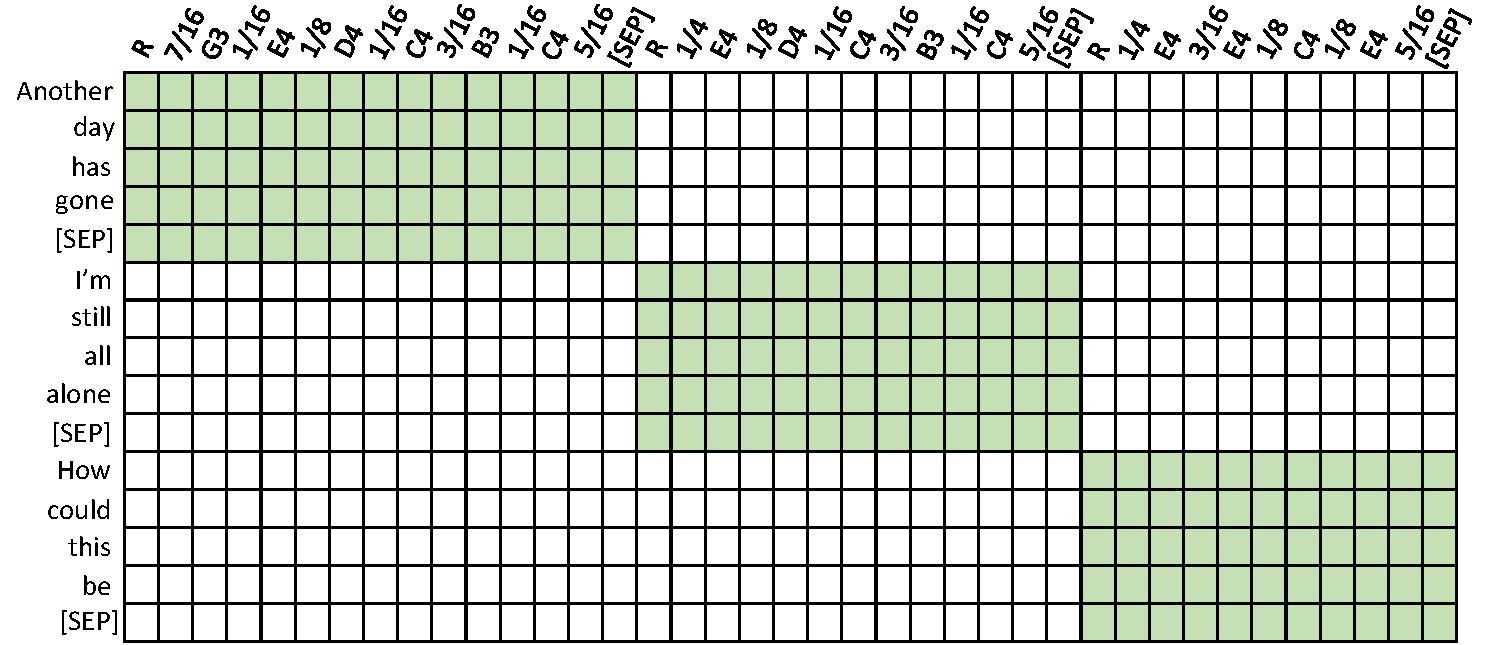
\includegraphics[width=0.99\textwidth]{figure/related/digattn.pdf}
  \caption{歌词和旋律之间的注意力权重矩阵示意图。}
  \label{fig:attn_diag}
\end{figure}
\begin{figure}[ht]
  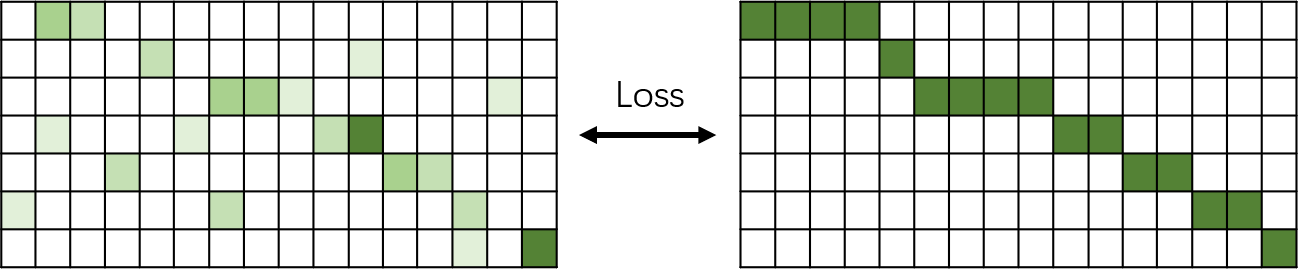
\includegraphics[width=0.99\textwidth]{figure/related/GuidedAttention.png}
  \caption{真实的对齐情况可以对歌词和旋律之间的注意力权重矩阵进行监督。}
  \label{fig:attn_loss}
\end{figure}
通过在注意力权重值的矩阵上进行动态规划求得最短路来找到歌词旋律之间合适的对齐方式。注意力矩阵本身除了相应任务的监督以外,也会受到真实对齐方式的监督。
然而,由于这种方法得出的对齐路径来自于某种对齐距离矩阵,在未加限制的情况下有时会导致一音符对齐多字的非单调性输出,并且自注意力机制模块在训练中也需要相对大量的数据。但最重要的一点可能是,这种方法的对齐组件是在得到翻译结果后提供类似基于规则的固定约束,而不是在训练期间和翻译一起动态地学习对齐的继承,即类似于后处理网络,而不是动态学习对齐从而限制歌词生成的模块。

\subsubsection{自适应计算时间}
本文在后文中使用的自适应分组的做法实际上是自适应计算时间算法的变种。自适应计算时间方法是\citet{act}中提出的,用于控制循环神经网络模型中每一个时刻重复运算的次数的算法,即使用算法来控制循环神经网络在时序顺序上的每一个时间步状态时的计算网络的深度。
\begin{figure}[ht]
  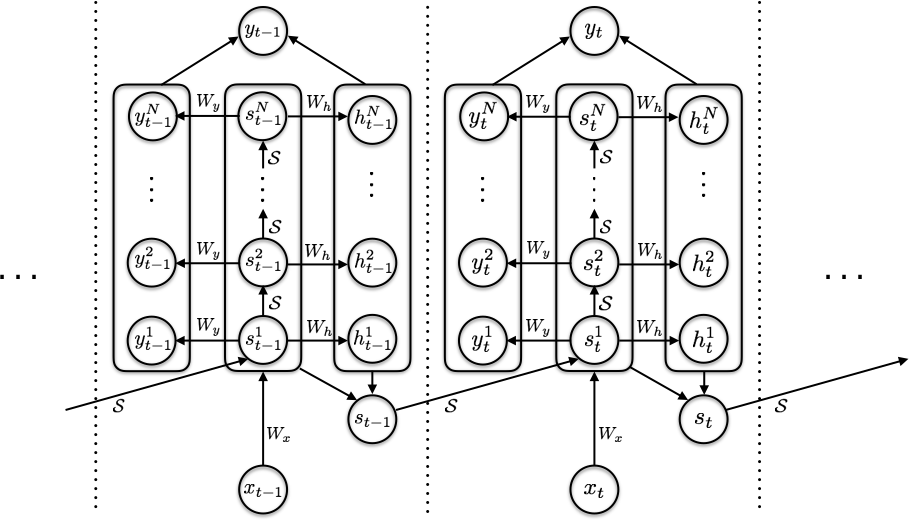
\includegraphics[width=0.99\textwidth]{figure/related/act.png}
  \caption{自适应计算时间控制循环神经网络的示意图。}
  \label{fig:act_rnn}
\end{figure}


本文提出的模型框架则是利用了歌词旋律对齐排列的单调性,进而设计了一个用于与翻译过程并行的进行对齐预测的轻量的神经网络。
\section{语音合成声学模型和扩散模型相关研究介绍}
\subsection{语音合成和歌声合成声学模型相关研究介绍}
\label{sec:svs_intro}
歌声合成研究起步于使用连接式的方法~\citep{macon1997concatenation,kenmochi2007vocaloid}或基于隐马尔可夫过程的参数化~\citep{saino2006hmm,oura2010recent}方法来生成声音。这两类方法在现在看来,流程都相对繁琐,且在内容上缺乏灵活性,音频听起来也不够和谐。由于深度学习的快速发展,在过去几年中,已经有多种基于深度神经网络的歌声合成系统被提出。\citet{nishimura2016singing,blaauw2017neural,kim2018korean,nakamura2019singing,gu2020bytesing}等工作率先尝试使用利用神经网络将上下文特征映射为声学参数特征。
基于深度神经网络的合成方法大致可以分成自回归和非自回归两类。
\subsubsection{时序自回归式的声学模型}
自回归类模型被提出的较早,其利用序列建模的方法,使用LSTM等循环神经网络对声音信号的线性频谱或梅尔频谱进行时序建模,一帧一帧地预测频谱的高低频情况。这一类模型的代表作就是Tacotron系列。
\begin{figure}[htbp]
  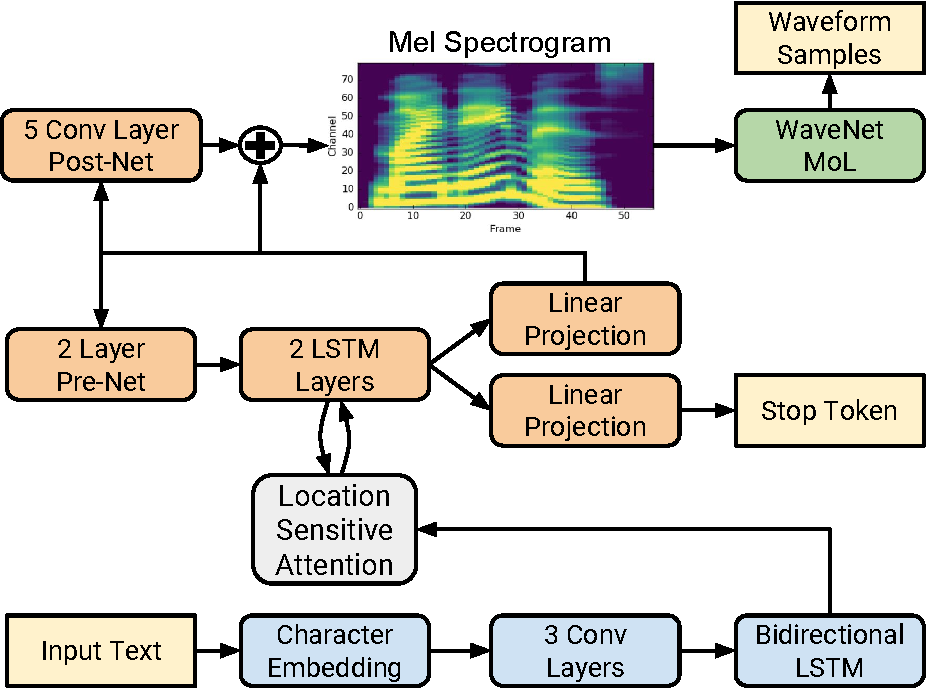
\includegraphics[width=0.99\textwidth]{figure/related/tacotron2.pdf}
  \caption{Tacotron声学模型示意图}
\end{figure}
Tacotron\citep{tacotron}构建的基于注意力机制的编码器-解码器框架将字符作为输入并输出线性频谱,使用Griffin-Lim算法\citep{GriffinLim}生成波形。Tacotron 2\citep{shen2018natural}则开始生成后续工作普遍采用的梅尔频谱并使用WaveNet\citep{vanwavenet}模型作为声码器并将梅尔频谱转换为波形。Tacotron 2和早期的连接式、参数式方法相比,合成的语音质量已经有了很大的提高。
后来也有许多工作尝试从不同方面改进和发展Tacotron系列。比如\citet{gsttacotron}、\citet{reftacotron}等在Tacotron原有框架基础上引入音频参考编码器和样式词来增强语音合成的表达能力。
\citet{nonattentivetacotron}和\citet{durian}则尝试替换Tacotron中的注意力机制,而使用一个单独的持续时间预测器进行自回归预测。
也有基于Tacotron构建端到端的文本直接生成波形的模型,如Wave Tacotron\citep{wavetacotron}。
基于Transformer结构的模型的提出最直接的动机就是使用循环神经网络构建的自回归模型有无法同时平行地训练和推理带来的模型效率问题和长频谱下自回归模型建模能力衰减的问题。
\begin{figure}[htbp]
  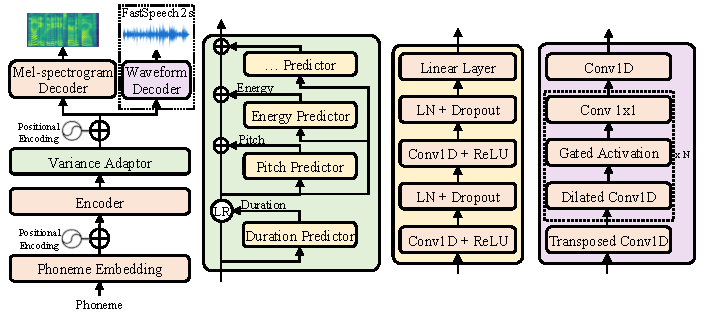
\includegraphics[width=0.99\textwidth]{figure/related/fs2.pdf}
  \caption{基于Transformer的声学模型示意图}
\end{figure}
\citet{transformertts}提出使用基于Transformer的编码器-解码器的基本模型结构来从输入的音素直接生成梅尔频谱。
\citet{transformertts}除了Transformer结构以外,仍沿用了Tacotron 2的一些设计,达到了和Tacotron 2的相似质量的音质,但训练和推理速度更快。然而,与基于循环神经网络Tacotron系列模型相比,Transformer中的编码器-解码器的注意力计算不够稳定和鲁棒,因此,一些工作开始致力于增强基于Transformer的声学模型的鲁棒性,如对注意力矩阵添加对角化限制\citep{robutrans}等。
但由于自回归本身的训练会带来暴露偏差(exposed bias)问题,这种建模方法有一定的缺陷,在实际应用中反映出的就是拖音、漏音、静音过长、韵律预测不稳等现象。
\subsubsection{非自回归式的声学模型}
非自回归类模型的提出相对较晚,但相关工作近来层出不穷,从基于Transformer结构的模型到基于各类生成模型的结构,有后来居上的趋势。
无论是Tacotron系列,还是基于Transformer的自回归模型,都存在上节提到的两个问题:推理速度慢和鲁棒性问题。
自回归的梅尔频谱生成速度较慢,特别是对于较长语音序列有较多的语音帧需要生成时。生成的语音存在一定的漏音、重复等造成音频听起来很不自然的问题,这主要是由基于Transformer的编码器-解码器的自回归生成中,文本和梅尔频谱之间的注意力对齐不准确造成监督不准确引起的。
因此\citet{ren2019fastspeech}
\begin{figure}[htbp]
  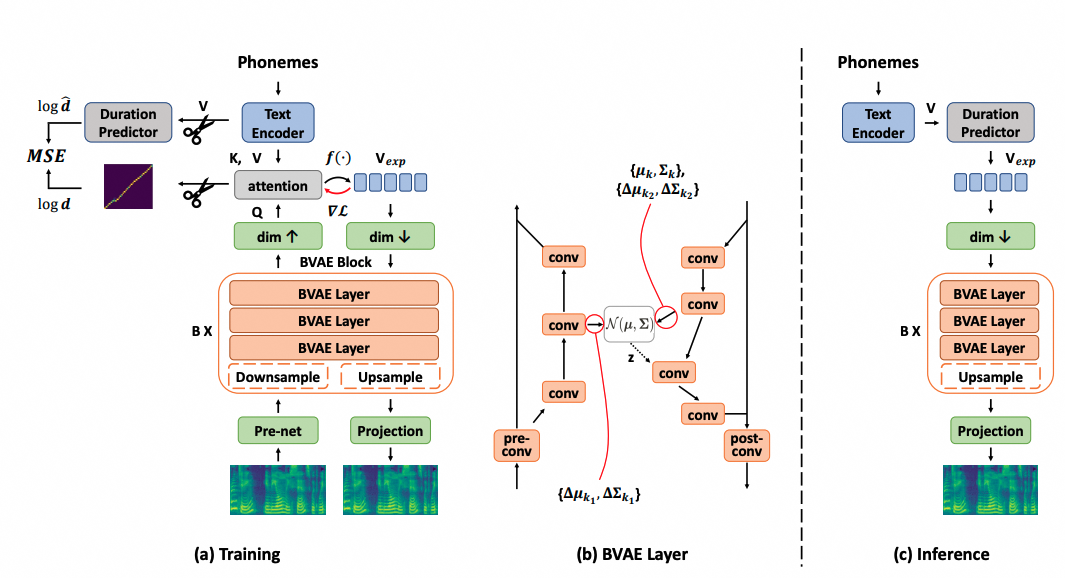
\includegraphics[width=0.99\textwidth]{figure/related/bvaetts.png}
  \caption{基于变分自编码器的声学模型示意图}
\end{figure}

\begin{figure}[htbp]
  \subfloat{
    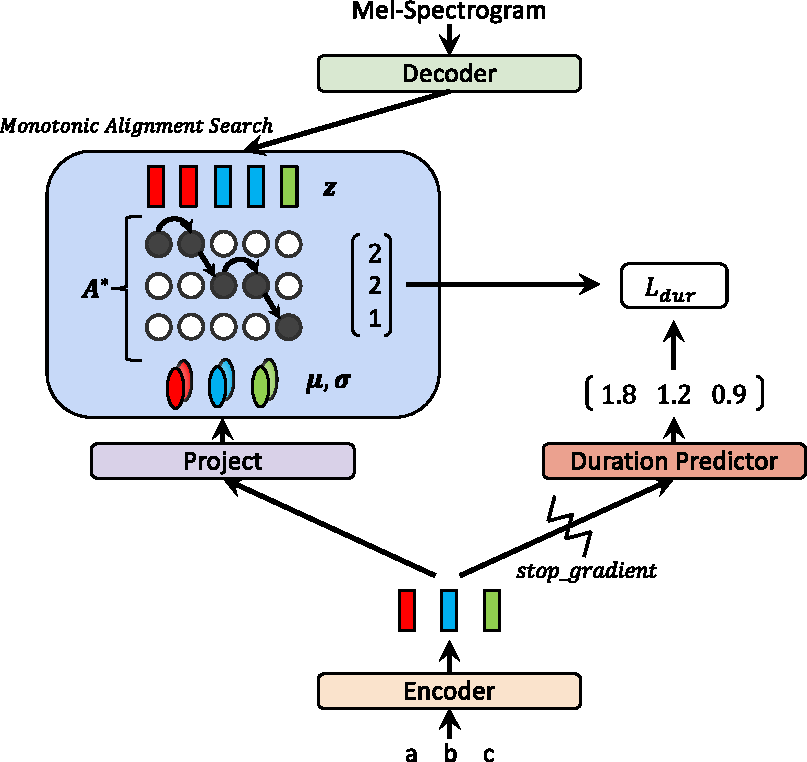
\includegraphics[width=0.49\textwidth]{figure/related/glowtts_a.pdf}
  }
  \subfloat{
    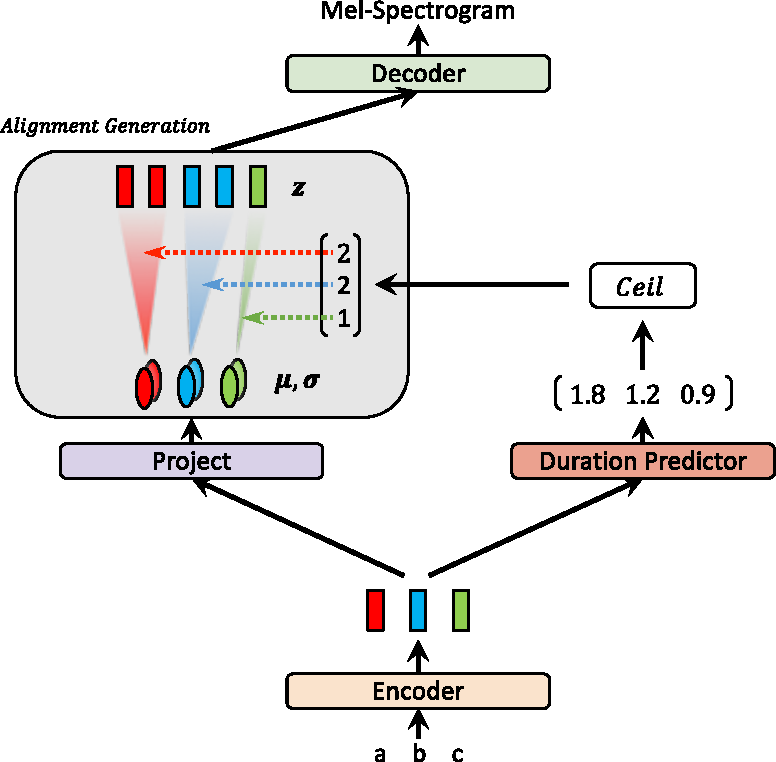
\includegraphics[width=0.49\textwidth]{figure/related/glowtts_b.pdf}
  }
  \caption{基于生成式流模型搭建的声学模型示意图}
\end{figure}

% \begin{figure}[htbp]
%   \includegraphics[width=0.99\textwidth]{figure/related/gantts.png}
%   \caption{基于生成对抗训练的声学模型示意图}
% \end{figure}
\subsection{歌声合成模型}
\citet{ren2020deepsinger}成功地使用了从音乐网站挖掘的歌唱数据从零开始构建了歌声合成系统,也为后续工作提供了一个方便的流程框架。\citet{blaauw2020sequence}则提出了一种基于前馈Transformer的非自回归歌声合成模型,推断过程快速,且能避免自回归模型引起的暴露偏差问题。
此外,对抗训练也是生成模型中的常用技术,在对抗训练的帮助下,\citet{lee2019adversarially}~提出了一个直接生成线性频谱的端到端框架。\citet{wu2020adversarially}~则提出了一个可以利用数量有限的录音数据就能构建起来的支持多歌手的歌声合成系统,并通过使用多随机窗口鉴别器来提高合成语音质量。\citet{chen2020hifisinger}~在模型中引入了多尺度对抗训练,以相对较高的采样率(48kHz)合成高清音频。
% \begin{figure}[htbp]
%   \includegraphics[width=0.99\textwidth]{figure/related/gantts.pdf}
%   \caption{基于对抗训练的歌声合成模型示意图}
% \end{figure}
近年来,歌声合成系统的音频结果的语音自然度和多样性都在不断提高,已显现在24kHz和48kHz下媲美人声的潜力。

\subsection{扩散模型相关研究介绍}
扩散概率模型也一种是通过优化似然函数整体变分下界进行训练的参数化的马尔可夫链,这样一个参数化的随机过程能以恒定的时间步长生成与数据分布匹配的样本~\citep{Ho2020ddpm}。
扩散模型首先由\citet{sohl2015deep}一文在2015年提出,之后的工作\citet{Ho2020ddpm}~又对最初的扩散模型进行了改进,以使用特定的参数化方式生成高质量图像,也揭示了扩散模型与去噪梯度得分匹配之间的等价性~\citep{song2019generative,song2021scorebased}。
\begin{figure}[htbp]
  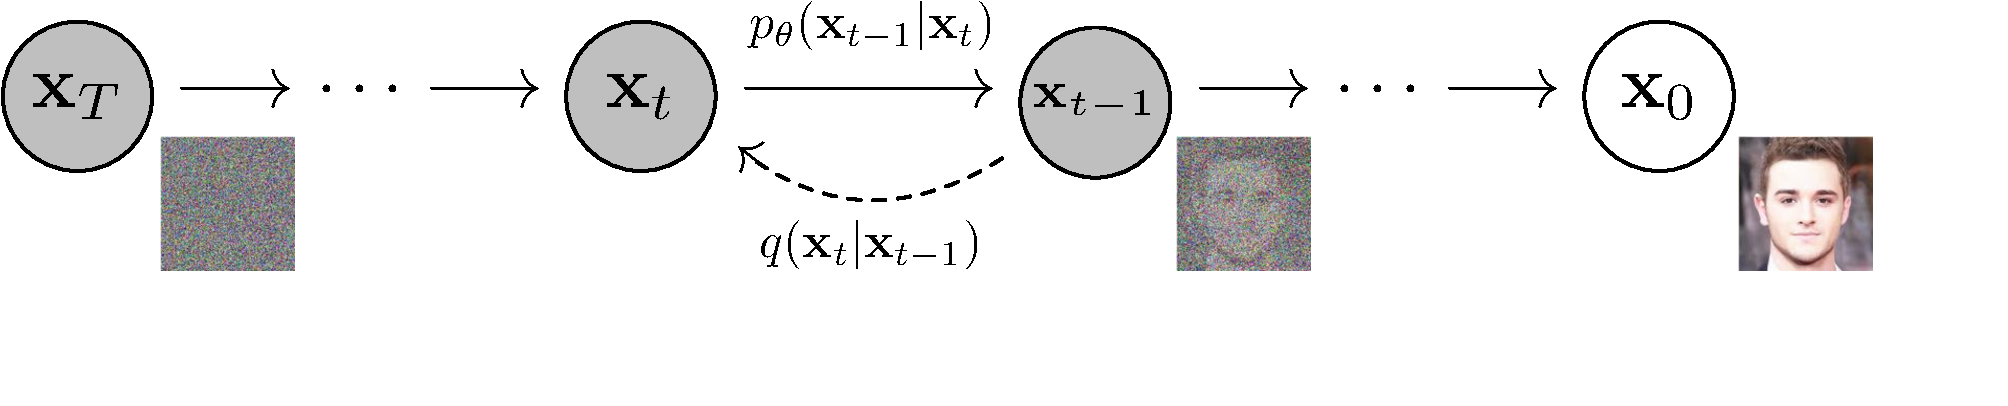
\includegraphics[width=0.99\textwidth]{figure/related/ddpm.pdf}
  \caption{基于扩散过程的图像去噪合成示意图}
\end{figure}
近来,随着扩散模型本身理论不断成熟,越来越多的工作开始尝试在应用任务中使用扩散模型来利用其高质量生成的优点并解决其运行速度慢的问题。\citet{kong2021diffwave}~和\citet{chen2021wavegrad}~两篇工作尝试将扩散模型应用于神经声码器这样的应用任务,根据梅尔频谱生成高保真的声音波形。
\begin{figure}[htbp]
  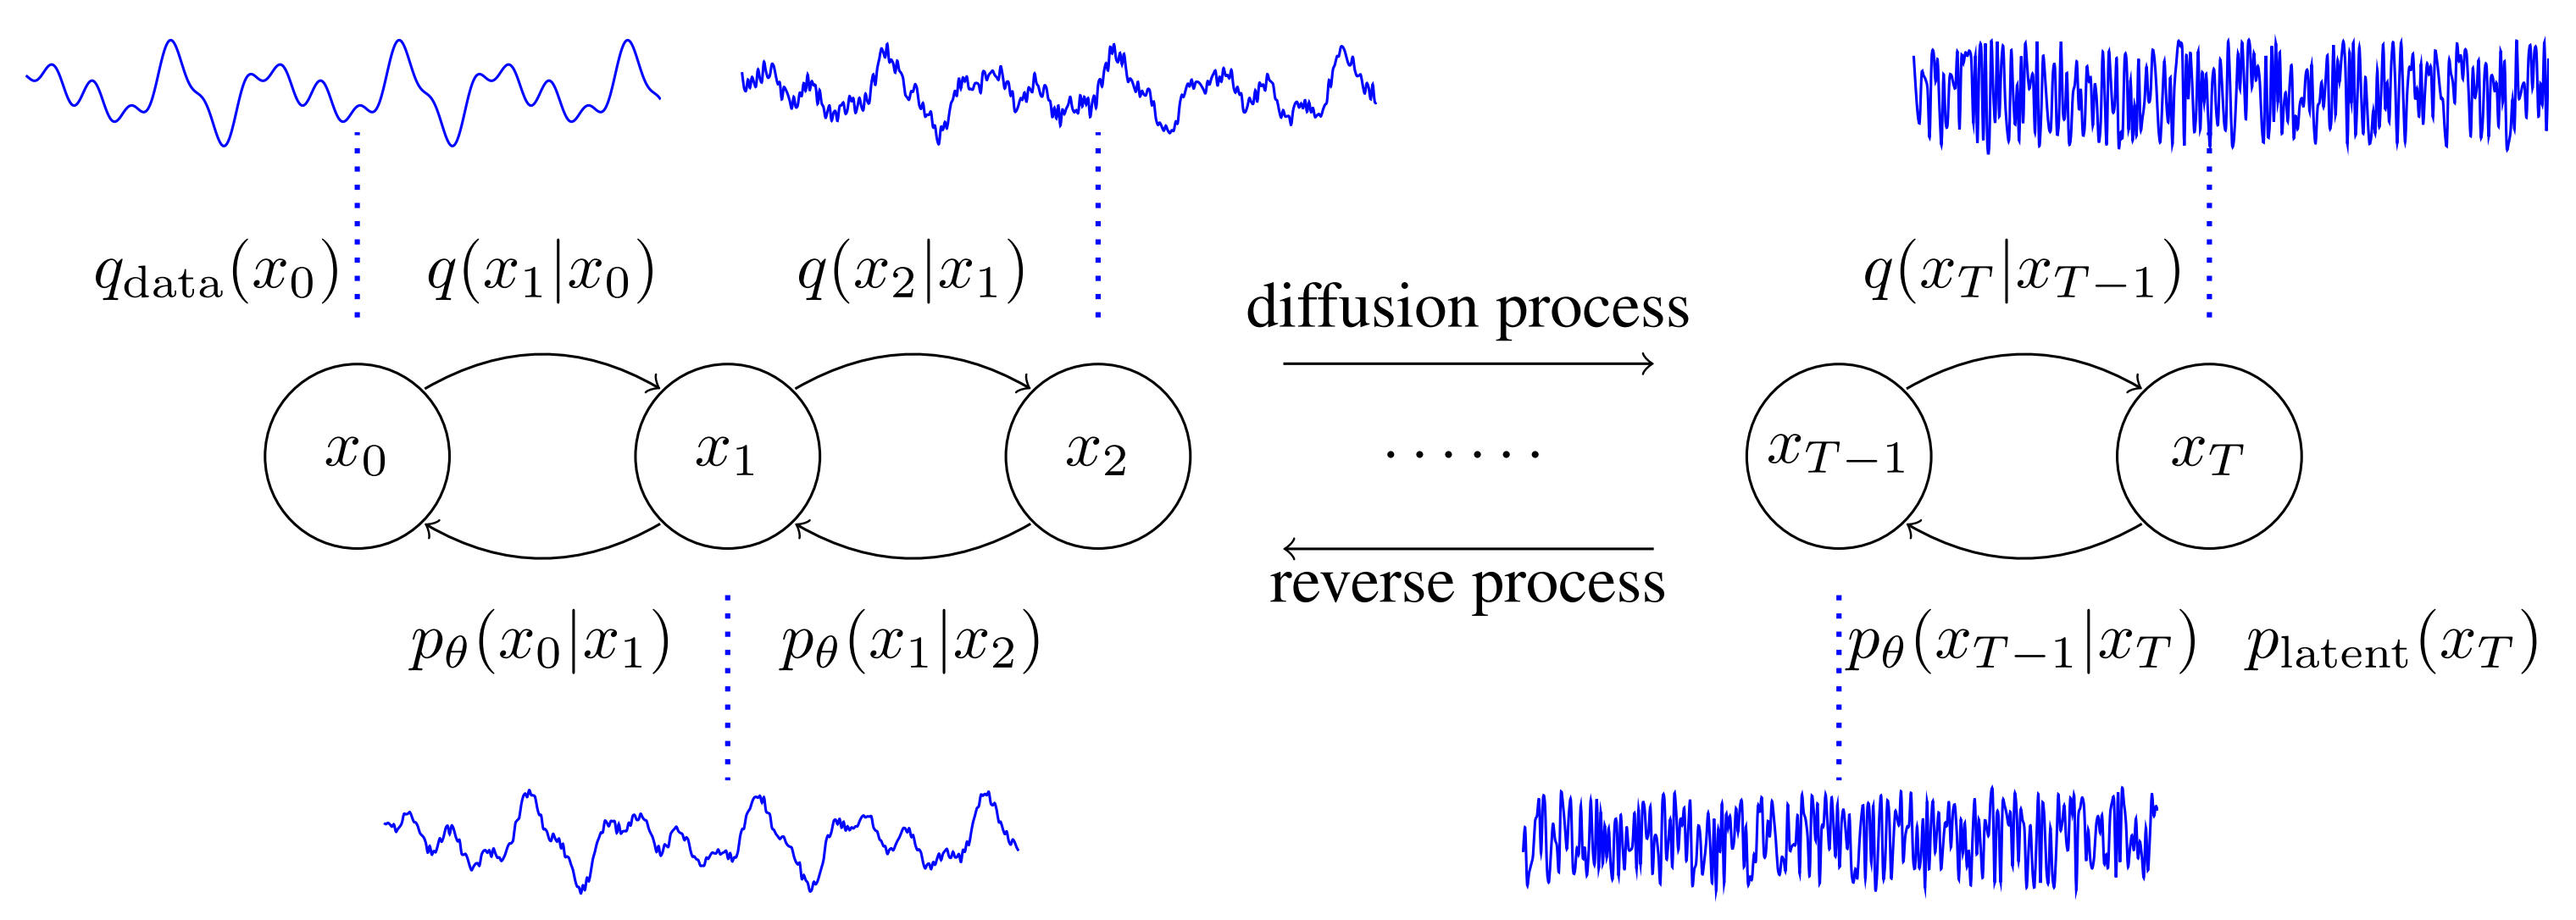
\includegraphics[width=0.99\textwidth]{figure/related/diffwave.png}
  \caption{基于扩散过程的声音波形合成示意图}
\end{figure}
\citet{chen2021wavegrad}~还提出了一种连续的噪声规划来减少推理迭代所需要的时间步数,同时保持原有的合成质量。\citet{song2021denoising}~通过提供更快的采样机制和有意义地在样本之间插值的方法来扩展扩散模型。扩散模型是一种新兴的技术,已应用于无条件图像生成、条件指导下的梅尔频谱到波形生成(神经声码器)等领域。在本文的工作中,\ref{sec:svs}节为提出了一个基于扩散模型声学模型,该模型在给定乐谱和文本(或仅给定文本)的情况下生成梅尔频谱。
\section{本章小结}
本章主要分多个领域分别介绍歌曲歌词生成及限制性翻译和歌声合成相关技术的背景、基本原理、国内外研究现状和近期进展。
